%*******************************************************************************
%*********************************** First Chapter *****************************
%*******************************************************************************

\chapter{Introduction}  %Title of the First Chapter
\label{ch:introduction}

\ifpdf
    \graphicspath{{Chapter1/Figs/Raster/}{Chapter1/Figs/PDF/}{Chapter1/Figs/}}
\else
    \graphicspath{{Chapter1/Figs/Vector/}{Chapter1/Figs/}}
\fi


%********************************** %First Section  **************************************
\section{Problem Background} %Section - 1.1
\label{sec:background}

Across modern industry, the controlled handling of fluids is fundamental to product quality, process efficiency, and operational safety. Processes in sectors such as food and beverage manufacturing, pharmaceuticals, wastewater treatment, and specialty chemicals all depend on the movement, blending, heating, and reaction of fluids under controlled conditions. In chemical engineering (ChE), these recurring processes are broadly classified as unit operations. Among them, agitation, or the mechanical mixing of fluids to improve uniformity and transfer processes, occupies a particularly important role because it influences reaction behavior, mass transfer, and heat transfer~\citep{paul2004,harnby2000}.

Because these operations are central to industrial practice, ChE education must do more than present them as abstract theory. Students must also be given opportunities to observe process behavior, collect experimental data, and interpret real systems using established engineering concepts. For this reason, laboratory instruction remains a core component of ChE curricula and an important bridge between theoretical principles and industrial practice~\citep{feisel2005}. This emphasis is consistent with Kolb's experiential learning cycle, which frames meaningful learning as a progression through concrete experience, reflective observation, abstract conceptualization, and active experimentation~\citep{kolb1984}.

From this perspective, effective laboratory equipment should support not only demonstration, but also measurement, analysis, and experimentation. It should help students connect physical behavior with engineering models while exposing them to the practical realities of instrumentation, data acquisition, and controlled operation~\citep{saco2002,uyanik2018}. In practice, however, undergraduate laboratories often face constraints related to equipment cost, limited unit availability, aging apparatus, and the difficulty of providing repeated hands-on access to large classes. These constraints create a broader need for laboratory platforms that are accessible, repeatable, instrumented, and pedagogically flexible, as reflected both in the development of low-cost experimental platforms for vessel-based ChE instruction~\citep{nassar2011,ganley2015} and in compact instructional systems for instrumentation and feedback-control education~\citep{plett2023,rehg1998fie}.

Within this broader instructional setting, process control becomes an important complementary topic because it introduces students to how process variables are measured, compared against desired values, and regulated through final control elements in the presence of disturbances and system variation~\citep{seborg2017,ogata2010}. One of the most accessible feedback strategies for introductory laboratory instruction is on-off control, in which an actuator is switched fully ON or fully OFF depending on whether the measured variable falls below or rises above a specified threshold or hysteresis band~\citep{ogata2010,nise2020}. Despite its simplicity, on-off control, also known as bang-bang control, is pedagogically valuable because it allows students to observe feedback action, actuator switching, and limit-cycle behavior directly before progressing to more advanced continuous control methods~\citep{uyanik2018,astrom1985}.

Taken together, these conditions point to a broader instructional need: laboratory environments should not only illustrate core ChE concepts, but should also provide students with accessible, repeatable, and instrumented opportunities for experimentation. This need becomes even more significant when laboratory courses must support both process understanding and introductory control-oriented learning within practical institutional constraints.


%********************************** %Second Section  *************************************
\section{Statement of the Problem} %Section - 1.2
\label{sec:problem}

At the University of San Carlos (USC), two ChE laboratory courses reveal clear gaps in instrumentation, accessibility, and hands-on process experimentation that the existing equipment can no longer adequately address.

%----------------------------------- Subsection 1.2.1 ---------------------------------
\subsection{CHE 3214L: Chemical Engineering Laboratory Investigations 1} % 1.2.1
\label{subsec:che3214l}

CHE 3214L is a key laboratory course for ChE students at USC. Among its experiments, ``Agitation of Water in a Cylindrical Tank'' requires students to evaluate flow behavior, power consumption, mixing time, and scale-up relationships in agitated systems. The experiment is interpreted using two dimensionless parameters: the Reynolds number, which indicates the flow regime and degree of turbulence, and the Power number, which represents the agitation power requirement of the impeller system~\citep{rushton1950}.

The impeller Reynolds number is defined as
\begin{equation}
N_{Re} = \frac{\rho n D_i^2}{\mu}
\label{eq:reynolds}
\end{equation}
where $N_{Re}$ is the Reynolds number (dimensionless), $\rho$ is the fluid density (\si{kg/m^3}), $n$ is the impeller rotational speed (rev/s), $D_i$ is the impeller diameter (m), and $\mu$ is the dynamic viscosity (\si{Pa.s}). 
The Power number is defined as
\begin{equation}
N_{Po} = \frac{P}{\rho n^3 D_i^5}
\label{eq:power}
\end{equation}
where $N_{Po}$ is the Power number (dimensionless) and $P$ is the impeller power consumption (W). These parameters are used to compare experimental agitation data against published $N_{Re}$--$N_{Po}$ correlation curves for standard impeller geometries established by Rushton, Costich, and Everett~\citep{rushton1950} and tabulated by Brown et al.~\citep{brown1950}.

\nomenclature[a-NRe]{$N_{Re}$}{Reynolds number, dimensionless}
\nomenclature[a-NPo]{$N_{Po}$}{Power number, dimensionless}
\nomenclature[a-P]{$P$}{Impeller power consumption [W]}
\nomenclature[a-n]{$n$}{Impeller rotational speed [rev/s]}
\nomenclature[a-Di]{$D_i$}{Impeller diameter [m]}
\nomenclature[g-rho]{$\rho$}{Fluid density [kg/m$^3$]}
\nomenclature[g-mu]{$\mu$}{Dynamic viscosity [Pa$\cdot$s]}

The sole apparatus for this experiment is the Armfield CEK-A Mixing and Agitation Unit~\citep{armfield2000}, shown in Fig.~\ref{fig:cek-a}. It is a floor-standing unit (approximately \SI{100}{kg}; \SI{820}{mm} $\times$ \SI{400}{mm} $\times$ \SI{860}{mm}) with a \SI{25}{L} acrylic tank (\SI{288}{mm} inner diameter), a variable-speed DC motor (0--500~rpm), open-loop speed control through a speed knob, an analog tachometer for speed indication, and a spring dynamometer for indirect torque estimation. It was purchased circa 2000 at Php~525,700.00 (Php~1,100,645.58 in 2023 terms~\citep{towler2013}; see Appendix~\ref{app:calculations}). After more than two decades of service, the unit exhibits several critical deficiencies.

% TODO: verify the CEPCI base year. Appendix A uses 1995 (CI = 381.1) but the text says the unit was bought circa 2000.

\begin{figure}[htbp]
    \centering
    % Place the CEK-A photo with annotations A, B, C in Chapter1/Figs/
    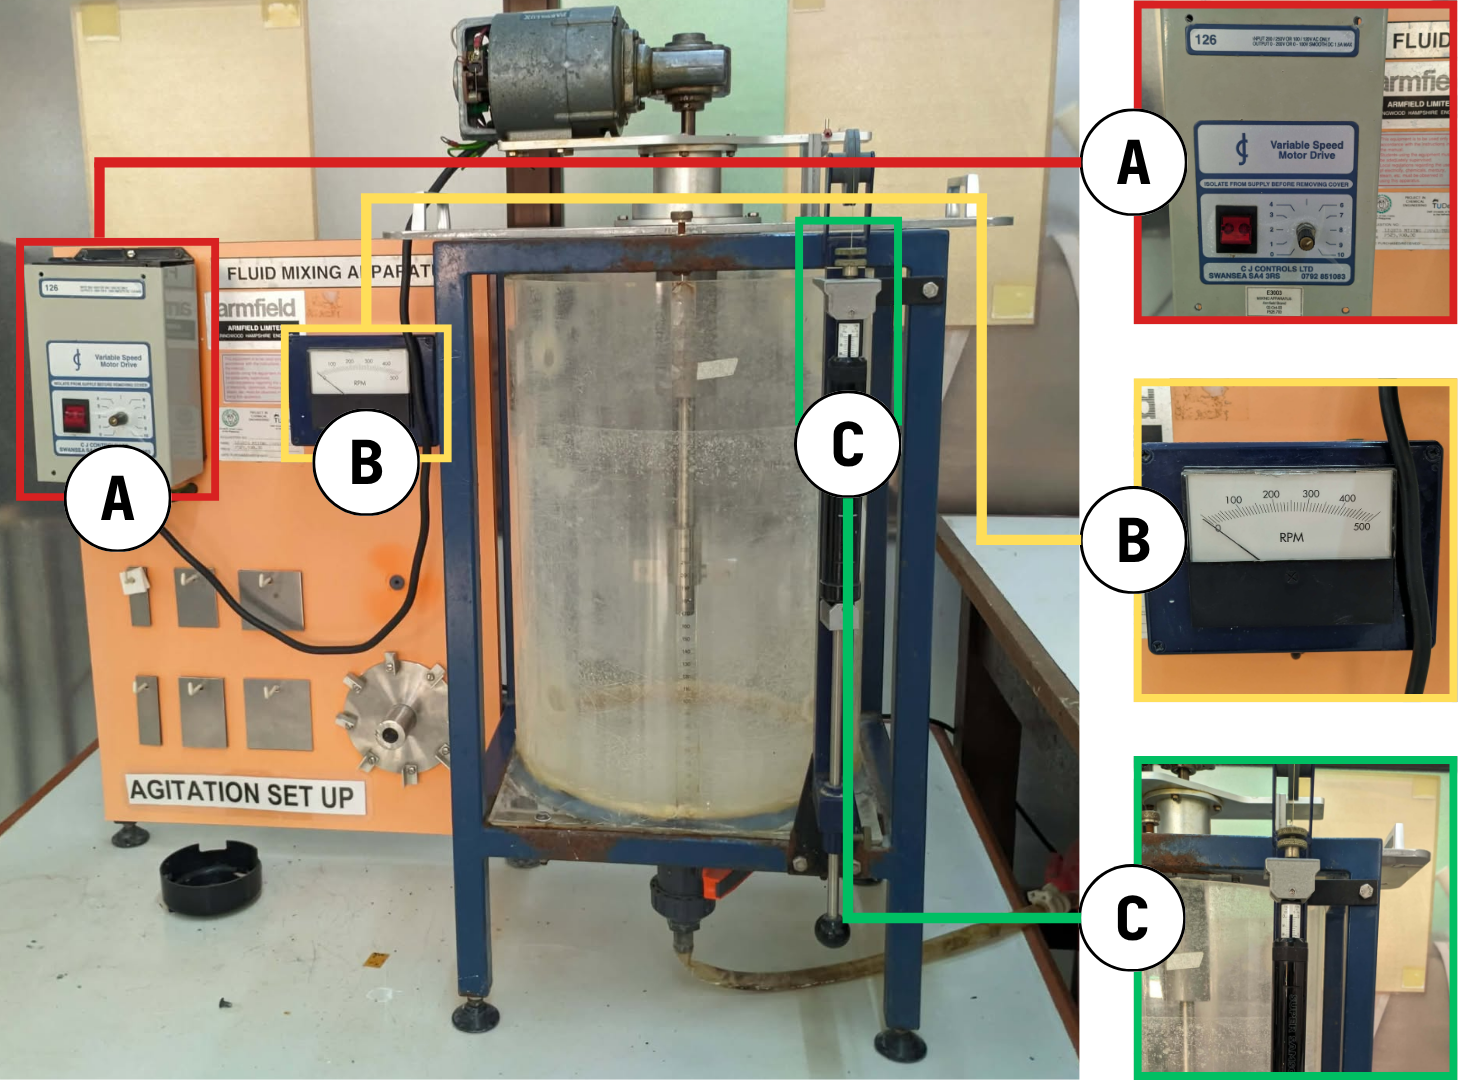
\includegraphics[width=0.7\textwidth]{cek-a-annotated}
    \caption[Armfield CEK-A Mixing and Agitation Unit]{Armfield CEK-A Mixing and Agitation Unit used in CHE 3214L, showing annotated components: (A)~speed knob, (B)~tachometer, and (C)~dynamometer.}
    \label{fig:cek-a}
\end{figure}

The major limitations of the CEK-A are as follows:

\begin{itemize}
    \item \textbf{Open-loop speed setting.} Because there is no feedback sensor in the control loop, the speed knob (Fig.~\ref{fig:cek-a}A) does not correspond to a guaranteed or repeatable rpm value. Students must manually search for the knob position that brings the impeller to the target speed, then verify the achieved rpm from the tachometer at each operating point.
    \item \textbf{Tachometer correction.} The analog tachometer (Fig.~\ref{fig:cek-a}B) is inaccurate in the 50--160~rpm range, and the laboratory manual prescribes the empirical correction
    \begin{equation}
    N_{\text{actual}} = 1.26 \times N_{\text{reading}} - 40.84
    \label{eq:tach-correction}
    \end{equation}
    which adds a manual conversion step and introduces further human error.
    \item \textbf{Indirect torque estimation.} Torque is not measured directly. Students read force from the spring dynamometer (Fig.~\ref{fig:cek-a}C), typically in grams or newtons, and then estimate torque from the torque-arm geometry. At low loads, small changes in force are difficult to distinguish reliably, and oscillation of the analog reading can make steady values harder to obtain.
    \item \textbf{Manual data gathering.} All measurements (speed, force, water level, and time) are recorded manually, making data collection time-consuming and error-prone~\citep{feisel2005}.
    \item \textbf{Geometric mismatch.} Because the CEK-A geometry does not closely match any standard configuration in the Brown et al.\ correlation table, students must rely on a near-match for the $N_{Re}$--$N_{Po}$ validation step, introducing ambiguity in interpreting observed discrepancies.
    \item \textbf{Repair constraints.} Repair is not feasible because the manufacturer no longer produces this model, proprietary parts are unobtainable, and retrofitting the tightly enclosed housing with digital sensors risks damaging the department's only working apparatus.
    \item \textbf{Commercial replacement limitations.} The commercial replacement, the Armfield CEK-MKII~\citep{armfield2023}, carries a quoted cost of up to Php~2.5 million. Its bundled armSOFT aLITE software can log mixer speed and torque, calculate mixer power, display data in real time, and generate graph plots for export. However, it operates as a proprietary black box that does not expose raw sensor data or support MATLAB/Simulink integration for hardware-in-the-loop (HIL) applications. At that price, the department would still receive only a single unit, leaving CHE 3214L students sharing one apparatus and CHE 4117L without a usable process plant.
\end{itemize}

\nomenclature[z-HIL]{HIL}{Hardware-in-the-Loop}
\nomenclature[z-ChE]{ChE}{Chemical Engineering}
\nomenclature[z-USC]{USC}{University of San Carlos}

%----------------------------------- Subsection 1.2.2 ---------------------------------
\subsection{CHE 4117L: Analysis and Design of Process Control Systems Laboratory} % 1.2.2
\label{subsec:che4117l}

CHE 4117L accompanies the lecture course CHE 4117 and is intended to develop students' ability to implement and evaluate feedback control systems on physical hardware. According to the long-time ChE laboratory custodian, the legacy process control rigs shown in Fig.~\ref{fig:legacy-4117} have been decommissioned for more than two decades due to age, escalating maintenance costs, and unavailability of compatible parts and software. As a result, CHE 4117L has been conducted entirely through MATLAB/Simulink simulations on desktop computers.

\begin{figure}[htbp]
    \centering
    % Place the four-panel photo of the legacy rigs in Chapter1/Figs/
    %\includegraphics[width=\textwidth]{legacy-che4117l}
    \caption[Legacy CHE 4117L process control equipment]{Legacy CHE 4117L process control equipment: (A)~Armfield PCT-14 process controller, (B)~Armfield PCT-13 temperature control unit, (C)~Armfield PCT-9 process module, and (D)~Armfield PCT-10/12 serial communications control accessory.}
    \label{fig:legacy-4117}
\end{figure}

While simulation is an essential component of control education~\citep{astrom1985}, exclusive reliance on it has well-documented shortcomings~\citep{ma2006}:

\begin{itemize}
    \item \textbf{No sensor noise or quantization.} Simulated signals are idealized, so students do not encounter the noise floors, quantization errors, or calibration drift associated with real sensors.
    \item \textbf{No actuator saturation or dead zones.} Simulated actuators typically respond linearly and instantaneously, whereas real motors, valves, and pumps exhibit slew-rate limits, backlash, and stiction.
    \item \textbf{No process disturbances.} Simulated disturbances are mathematical injections into a transfer function, whereas real disturbances, such as accidental tank disturbances or changes in water supply conditions, are less predictable and require more robust controller design.
\end{itemize}

The absence of a physical process plant therefore limits hands-on learning in CHE 4117L and represents a curricular gap with respect to Outcomes-Based Education frameworks that expect students to engage with real hardware and modern engineering tools~\citep{ptcacbet2023,ched2017che}.

Taken together, these conditions motivate the need for an accessible and digitally instrumented laboratory platform that can support both agitation experimentation and introductory process-control activities. Related work by Dumalagan has already established the mechanical design basis of a low-cost countertop fluid mixing apparatus, referred to in this study as the Mixing Instrumentation eXperimental Rig~1 (MIXR-1)~\citep{dumalagan2024}. Accordingly, this study focuses on the Computer Engineering (CpE) side of that platform, specifically the digitally instrumented and computer-integrated subsystems needed to make MIXR-1 suitable for modern data acquisition and introductory process-control instruction.

\nomenclature[z-MIXR1]{MIXR-1}{Mixing Instrumentation eXperimental Rig 1}
\nomenclature[z-CpE]{CpE}{Computer Engineering}


%********************************** % Third Section  *************************************
\section{Goals and Objectives}  %Section - 1.3
\label{sec:objectives}

Confronted with aging laboratory hardware, the high cost of commercial replacements, and the lack of physical systems for hands-on learning in agitation operations and process control, this study adopts a design-oriented approach from the computer engineering perspective. It aims to support the improvement of chemical engineering laboratory education through the development of a low-cost, serviceable, and digitally instrumented mixing apparatus that can interface with MATLAB/Simulink.

In line with this aim, the study pursued the following specific objectives:

\begin{enumerate}
    \item To design and integrate the sensing, signal-conditioning, and control hardware required for the MIXR-1 fluid mixing apparatus.
    \item To develop the software stack required for three operating modes: a standalone LCD-based mode, a PC dashboard mode with visualization and data export, and a MATLAB/Simulink-integrated hardware-in-the-loop mode.
    \item To implement the core agitation experiments and introductory process-control functions required for CHE 3214L and CHE 4117L laboratory activities, with validation based on defined system-level performance tests, comparative analysis, and error measurements.
\end{enumerate}

The project deliverables corresponding to each objective are tabulated in Appendix~\ref{app:deliverables}.


%********************************** % Fourth Section  *************************************
\section{Significance of the Study}  %Section - 1.4
\label{sec:significance}

\subsection{For Students} % 1.4.1

MIXR-1 provides CHE 3214L with a digitally instrumented replacement for the aging CEK-A, eliminating open-loop speed control, empirical tachometer correction, low-resolution torque estimation, and fully manual data gathering while preserving the standard $N_{Re}$--$N_{Po}$ and mixing-time experiments specified in the laboratory manual. This makes it more practical to obtain repeatable hydrodynamic data and shifts student effort from transcription and error-prone calculation toward interpreting mixing behavior and scale-up relationships.

For CHE 4117L, the prototype reintroduces a physical process plant to a laboratory that has operated purely in simulation since the legacy rigs were decommissioned. Students gain a platform that supports on-off water-level regulation via MATLAB/Simulink, reconnecting control-design work with the nonidealities of real sensors, actuators, and disturbances.

\subsection{For Higher Education Institutions} % 1.4.2

For USC, MIXR-1 offers a low-cost, serviceable alternative to both retrofitting the CEK-A and purchasing a CEK-MKII at up to Php~2.5 million with closed armSOFT aLITE software and no Simulink integration. With a materials cost of approximately Php~50,000 per unit (Appendix~\ref{app:cost}), a budget comparable to a single CEK-MKII acquisition could instead support multiple MIXR-1 units, enabling parallel operation by several student groups and easing the accessibility and throughput issues currently faced in CHE 3214L and CHE 4117L.

% TODO: update the per-unit cost after the as-built BOM is final (the torque sensor, motor driver, and ToF sensor changed from the proposal BOM, which totaled Php 50,151.98).

Because the system is built on a Raspberry Pi platform with Ethernet connectivity and the official MATLAB/Simulink support package~\citep{mathworks2026}, it aligns with outcomes-based expectations for modern engineering tools and creates an extensible baseline for subsequent cohorts to add sensors, control schemes, and experiments without vendor lock-in.

\subsection{For the Broader Engineering Education Community} % 1.4.3

More broadly, MIXR-1 contributes to existing work on low-cost, open laboratory platforms by combining an agitated mixing vessel, embedded motor control, on-off level control, and MATLAB/Simulink connectivity in a design reproducible from commonly available components. Institutions facing aging agitation rigs, discontinued control equipment, or overreliance on simulation may adapt the electronic architecture and three-mode software concept to their own mechanical baselines, using MIXR-1 as a template for interdisciplinary collaboration between chemical and computer engineering programs in resource-constrained settings.


%********************************** % Fifth Section  *************************************
\section{Scope and Limitations}  %Section - 1.5
\label{sec:scope}

\subsection{Scope} % 1.5.1
\label{subsec:scope}

The scope of this study covers the following:

\begin{enumerate}
    \item The study focuses solely on the computer engineering aspects of the MIXR-1 project, specifically the electronics, circuitry, embedded systems, software, data acquisition, and control aspects. The electronic components and circuitry are based on the hardware stipulated in the work of Dumalagan~\citep{dumalagan2024}, together with the additional hardware required to implement water-level on-off control, while the mechanical and chemical engineering design of the system is adopted as a fixed design input.
    \item The study implements the MIXR-1 computer-engineering subsystems only, limited to interfacing the selected sensors and actuators with the Raspberry Pi, implementing the on-board control routines, and providing the minimum local interface and MATLAB/Simulink link needed to run the target laboratory experiments.
    \item Sensor interfacing includes only the sensors and display modules required to support the intended data acquisition, monitoring, and control functions of the system.
    \item Data acquisition and motor control are managed by the Raspberry Pi single-board computer, with low-level acquisition and higher-level application functions implemented for computation, display, logging, and communication. Proportional-integral (PI) speed control is implemented as an embedded function by the proponents, while on-off water-level control is designed and deployed by students via MATLAB/Simulink hardware-in-the-loop operation.
    \item The graphical user interface is limited to the three core interfaces required for the deliverables: standalone local operation via LCD and push buttons, PC dashboard visualization and data logging, and MATLAB/Simulink hardware-in-the-loop operation.
    \item Experimental implementation is aligned with the experimental conditions and procedures described in the official USC Department of Chemical Engineering laboratory manual for the target laboratory activities.
    \item The system is brought to a prototype state through internal unit testing, integration testing, comparative performance testing, and percentage-error analysis conducted by the proponents and, where applicable, with the guidance of Engr.\ Dumalagan.
    \item Demonstrated functionality includes internal testing of CHE 3214L-related activities such as agitation, $N_{Re}$--$N_{Po}$ generation, and mixing-time measurement, as well as the CHE 4117L-related activity of on-off water-level control via MATLAB/Simulink hardware-in-the-loop operation. The results are compared with the old laboratory system, independent measuring instruments, and available laboratory reference data to show measurable performance differences.
    \item The comparative analysis uses established engineering and laboratory parameters, including steady-state speed error, speed-setpoint tracking, torque and power measurement error, water-level measurement error, data-logging completeness, and integration with MATLAB/Simulink.
    \item The percentage-error analysis is computed using independent references such as a handheld tachometer, a physical ruler for measuring the actual water level, theoretical torque computation, a digital multimeter, laboratory manual values, existing chemical-engineering laboratory datasets, or another advisor-approved reference system when available.
    \item Communication between the Raspberry Pi and the host PC is implemented over wired TCP/IP via Gigabit Ethernet.
\end{enumerate}

\subsection{Limitations} % 1.5.2
\label{subsec:limitations}

The limitations of this study are as follows:

\begin{enumerate}
    \item The study does not consider experimental conditions, procedures, or operating ranges beyond those specified in the official USC Department of Chemical Engineering laboratory manual for the relevant experiments; laboratory manuals or experimental protocols from other institutions are not adopted.
    \item Advanced control strategies, including full PID control, model predictive control (MPC), adaptive control, and cascade control, are not implemented. Control does not go beyond PI speed regulation, implemented as an embedded function by the proponents, and on-off water-level control, designed and deployed by students via Simulink.
    \item Wi-Fi communication is not implemented; communication between the Raspberry Pi and the host PC is limited to wired TCP/IP over Gigabit Ethernet.
    \item Hardware configurations other than those stipulated in Dumalagan~\citep{dumalagan2024} and the additional components required for water-level on-off control are not considered.
    \item The graphical user interface does not include features beyond the three core interfaces defined in the scope. Extended export workflows, more elaborate dashboard structures, and nonessential analysis utilities are outside the scope of this study.
    \item Full deployment of MIXR-1 as an official CHE 3214L or CHE 4117L experiment for regularly scheduled class use falls outside this study.
    \item User-feedback studies, usability evaluations, and classroom beta testing are not conducted within this study and are recommended as future work (Section~\ref{sec:recommendations}).
    \item Long-term reliability testing, multi-semester deployment, maintenance studies, and broader field use are not part of this study; the immediate focus is to deliver a fully working prototype with validated core experimental and control functions through internal testing.
    \item The comparative analysis is limited to accessible data from the existing laboratory system, official laboratory procedures, available chemical-engineering laboratory records, and independent reference instruments. If the old system cannot be operated safely or completely, comparison is made using documented specifications, historical laboratory data, and advisor-approved reference measurements.
    \item Error analysis quantifies measurement and control deviations within the prototype testing conditions only. It does not claim certification-grade accuracy, long-term calibration stability, or performance under operating ranges outside those defined in the study.
\end{enumerate}

\nomenclature[z-PI]{PI}{Proportional-Integral}
\nomenclature[z-PID]{PID}{Proportional-Integral-Derivative}
\nomenclature[z-MPC]{MPC}{Model Predictive Control}
\nomenclature[z-SBC]{SBC}{Single-Board Computer}
\nomenclature[z-GUI]{GUI}{Graphical User Interface}


%********************************** % Sixth Section  *************************************
\section{Organization of the Thesis}  %Section - 1.6
\label{sec:organization}

This thesis is organized top-down by system function. After the introductory, literature, and architecture chapters, the shared electronics and embedded software are presented first, followed by one chapter for each experimental application of the platform.

Chapter~\ref{ch:rrl} reviews related literature on process control education, low-cost agitation apparatus, low-cost process control kits, and embedded and open-source hardware in education, and identifies the research gap addressed by this work. Chapter~\ref{ch:system} gives a high-level overview of the MIXR-1 system architecture, introducing the hardware, electronics, and software through block diagrams and signal-flow graphs, together with the communication protocols, development approach, and validation framework.

Chapter~\ref{ch:platform} presents the electronics and embedded software platform shared by all operating modes: power distribution, circuitry and the electronics enclosure, the Raspberry Pi~4B embedded core, the real-time backend daemon, hardware abstraction, timing and sampling, and the safety features and fault handling common to every mode. Chapter~\ref{ch:agitation} covers the agitation application used for CHE 3214L, grouping the rotary encoder, motor driver, PI speed control, torque sensing, the standalone local interface (Mode~1), the PC dashboard and data logging (Mode~2), and agitation validation. Chapter~\ref{ch:process} covers the process-control application used for CHE 4117L, grouping the time-of-flight level sensor, level-control actuation, the MATLAB/Simulink hardware-in-the-loop mode (Mode~3), the on-off level controller, and its validation. The two application chapters are kept separate so that agitation and process-control discussions do not overlap.

Chapter~\ref{ch:validation} reports system integration, validation, and the comparative analysis between MIXR-1 and the legacy Armfield CEK-A, including percentage-error analysis and error mitigation. Finally, Chapter~\ref{ch:conclusions} summarizes the study, presents the conclusions, and offers recommendations for future work. Supplementary calculations, schedules, cost estimates, test-case descriptions, schematics, preliminary test data, source code, and a user guide are provided in the appendices.